
\section{Case study: SAGE data} \label{zhang}
\subsection{Introduction}
This section provides a detailed analysis of data from a SAGE
experiment to illustrate the data analysis pipeline for \edgeR. The
data come from a very early study using SAGE technology to analyse
gene expression profiles in human cancer cells \citep{Zhang:1997p13}.

\subsection{Source of the data}
At the time that \citet{Zhang:1997p13} published their paper, no
comprehensive study of gene expression in cancer cells had been
reported. \citet{Zhang:1997p13} designed a study to address the
following issues:
\begin{enumerate}
\item How many genes are expressed differentially in tumour versus
  normal cells?
\item Are the majority of those differences cell-autonomous rather
  than dependent on the tumour micro-environment?
\item Are most differences cell type-specific or tumour-specific?
\end{enumerate}
They used normal and neoplastic gastro-intestinal tissue as a
prototype and analysed global profiles of gene expression in human
cancer cells. The researchers derived transcripts from human
colorectal (CR) epithelium, CR cancers or pancreatic cancers. The data
that we analyse in this case study are \citet{Zhang:1997p13}'s SAGE
results for the comparison of expression patterns between normal colon
epithelium and primary colon cancer.

They report that the expression profiles revealed that most
transcripts were expressed at similar levels, but that $289$
transcripts were expressed at significantly different levels
[$P$-value < 0.01] and that $181$ of these $289$ were decreased in
colon tumours as compared with normal colon
tissue. \citet{Zhang:1997p13} used Monte Carlo simulation to determine
statistical significance. In this case study we will use the
\edgeR~package, based around the negative binomial model, to identify
genes differentially expressed in the normal and cancer samples.


\subsection{Reading in the data and creating a \code{DGEList} object}
Our first task is to load the \edgeR~package, read the data into
\R~and organise the data into a \code{DGEList} object that the
functions in the package can recognise. The library size is usually
the total sum of all of the counts for a library, and that is how
library size is defined in this analysis. The easiest way to construct
an appropriate \code{DGEList} object for these data is described
below.

In this case, the tag counts for the four individual libraries are
stored in four separate plain text files, \code{GSM728.txt,
  GSM729.txt, GSM755.txt \textrm{and} GSM756.txt}. In each file, the
tag IDs and counts for each tag are provided in a table. It is best to
create a tab-delimited, plain-text `Targets' file, which, under the
headings `files', `group' and `description', gives the filename, the
group and a brief description for each sample.

The \code{targets} object is produced when the `Targets.txt' file is
read into the \R~session. This object makes a convenient argument to
the function \code{readDGE} which reads the tables of counts into our
\code{R} session, calculates the sizes of the count libraries and
produces a \code{DGEList} object for use by subsequent functions.

\begin{Schunk}
\begin{Sinput}
> library(edgeR)
> path <- getwd()
> setwd("/Users/dmccarthy/Documents/DGE/ZhangData")
> targets <- read.delim(file = "Targets.txt", stringsAsFactors = FALSE)
> targets
\end{Sinput}
\begin{Soutput}
       files group                description
1 GSM728.txt    NC               Normal colon
2 GSM729.txt    NC               Normal colon
3 GSM755.txt    Tu Primary colonrectal tumour
4 GSM756.txt    Tu Primary colonrectal tumour
\end{Soutput}
\begin{Sinput}
> d <- readDGE(targets, skip = 5, comment.char = "!")
> dim(d)
\end{Sinput}
\begin{Soutput}
[1] 57448     4
\end{Soutput}
\begin{Sinput}
> d
\end{Sinput}
\begin{Soutput}
An object of class "DGEList"
$samples
       files group                description lib.size norm.factors
1 GSM728.txt    NC               Normal colon    50179            1
2 GSM729.txt    NC               Normal colon    49593            1
3 GSM755.txt    Tu Primary colonrectal tumour    57686            1
4 GSM756.txt    Tu Primary colonrectal tumour    49064            1

$counts
              1    2    3   4
CCCATCGTCC 1288 1380 1236   0
CCTCCAGCTA  719  458  148 142
CTAAGACTTC  559  558  248 199
GCCCAGGTCA  520  448   22  62
CACCTAATTG  469  472  763 421
57443 more rows ...
\end{Soutput}
\begin{Sinput}
> setwd(path)
\end{Sinput}
\end{Schunk}

We will filter out very lowly expressed tags. Those which have fewer
than 5 tags in total cannot possibly achieve statisical significance
for DE, so we filter out these tags.

\begin{Schunk}
\begin{Sinput}
> d <- d[rowSums(d$counts) >= 5, ]
> dim(d)
\end{Sinput}
\begin{Soutput}
[1] 5012    4
\end{Soutput}
\begin{Sinput}
> d$samples$lib.size
\end{Sinput}
\begin{Soutput}
[1] 50179 49593 57686 49064
\end{Soutput}
\begin{Sinput}
> colSums(d$counts)
\end{Sinput}
\begin{Soutput}
    1     2     3     4 
34970 35764 36940 30325 
\end{Soutput}
\begin{Sinput}
> d$samples$lib.size <- colSums(d$counts)
> d <- calcNormFactors(d)
> d$samples
\end{Sinput}
\begin{Soutput}
       files group                description lib.size norm.factors
1 GSM728.txt    NC               Normal colon    34970    0.9757300
2 GSM729.txt    NC               Normal colon    35764    0.9654074
3 GSM755.txt    Tu Primary colonrectal tumour    36940    0.9706259
4 GSM756.txt    Tu Primary colonrectal tumour    30325    1.0937243
\end{Soutput}
\end{Schunk}

We see that the vast majority of tags sequenced in this experiment are
detected at very low levels. This filtering step reduces the dataset
from over 50,000 tags to just over 5000. While this may seem drastic,
there is simply no information for DE in the tags we have filtered
out. Nevertheless, the filtering reduces the library sizes (total
counts in each library) by about 30\%.

In the output above we also show the application of TMM normalization
to these data using the function \code{calcNormFactors}. The
normalization factors here are all very close to one, which indicates
that the four libraries are very similar in composition.

This \code{DGEList} is now ready to be passed to the functions that do
the calculations to determine differential expression levels for the
genes. Note that when we `see' the \code{DGEList} object \code{d}, the
counts for just the first five genes in the table are shown, as well
as the library sizes and groups for the samples.


\subsection{Analysis using common dispersion}
\subsubsection{Estimating the common dispersion}
The first major step in the analysis of DGE data using the NB model is
to estimate the dispersion parameter for each tag. The most
straight-forward analysis of DGE data uses the common dispersion
estimate as the dispersion for all tags. For many applications this
will be adequate and it may not be necessary to estimate tagwise
dispersions, i.e.~estimate the dispersion parameter separately for
each tag. Using the common dispersion allows the user to obtain DE
results very quickly and in few steps, and so makes a good place to
start with any analysis of DGE data.

Estimating the common dispersion is done using the function
\code{estimateCommonDisp}. In order to do this, the function first
needs to generate the `pseudocounts' under the alternative hypothesis
(that there really is a difference in expression level between the
groups). The conditional maximum likelihood method assumes that the
library sizes are equal, which is certainly not true in general for
DGE data.

The pseudocounts are calculated using a quantile-to-quantile method
for the negative binomial distribution so that the library sizes for
the pseudocounts are equal to the geometric mean of the original
library sizes. These pseudocounts are then used as the count data for
the common conditional negative binomial likelihood function, which is
maximised over the dispersion parameter to obtain our estimate of the
common dispersion.

\begin{Schunk}
\begin{Sinput}
> d <- estimateCommonDisp(d)
> names(d)
\end{Sinput}
\begin{Soutput}
[1] "samples"           "common.dispersion" "counts"           
[4] "pseudo.alt"        "genes"             "all.zeros"        
[7] "conc"              "common.lib.size"  
\end{Soutput}
\end{Schunk}

The output of \code{estimateCommonDisp} is a DGEList object with
several new elements. The element \code{common.dispersion}, as the
name suggests, provides the estimate of the common dispersion, and
\code{pseudo.alt} gives the pseudocounts calculated under the
alternative hypothesis. The element \code{genes} contains the
information about gene/tag identifiers. The element \code{conc} gives
the estimates of the overall concentration of each tag across all of
the original samples (\code{conc\$conc.common}) and the estimate of
the concentration of each tag within each group
(\code{conc\$conc.group}). The element \code{common.lib.size} gives
the library size to which the original libraries have been adjusted in
the pseudocounts.

We see in the output below that the total number of counts in each
library of the pseudocounts agrees well with the common library size,
as desired.

\begin{Schunk}
\begin{Sinput}
> d$samples$lib.size
\end{Sinput}
\begin{Soutput}
[1] 34970 35764 36940 30325
\end{Soutput}
\begin{Sinput}
> d$common.lib.size
\end{Sinput}
\begin{Soutput}
[1] 34404.07
\end{Soutput}
\begin{Sinput}
> colSums(d$pseudo.alt)
\end{Sinput}
\begin{Soutput}
       1        2        3        4 
35261.11 35637.21 35443.58 31458.46 
\end{Soutput}
\end{Schunk}

Under the negative binomial model, the square root of the common
dispersion gives the coefficient of variation of biological
variation. Here, as seen in the code below, the coefficient of
variation of biological variation is found to be $0.44$. We also note
that a common dispersion estimate of $0.2$ means that there is a lot
more variability in the data that can be accounted for by the Poisson
model---if a tag has just $200$ counts on average in each library,
then the estimate of the tag's variance under the NB model is over
$40$ times greater than it would be under the Poisson model.

\begin{Schunk}
\begin{Sinput}
> d$common.dispersion
\end{Sinput}
\begin{Soutput}
[1] 0.1968823
\end{Soutput}
\begin{Sinput}
> sqrt(d$common.dispersion)
\end{Sinput}
\begin{Soutput}
[1] 0.4437142
\end{Soutput}
\end{Schunk}

\subsubsection{Testing}
Once we have an estimate of the common dispersion, we can proceed with
testing procedures for determining differential expression. The
\edgeR~package uses an exact test for the negative binomial
distribution, which has strong parallels with Fisher's exact test, to
compute exact $p$-values that can be used to assess differential
expression. The function \code{exactTest} allows the user to conduct
the NB exact test for pairwise comparisons of groups. Here there are
only two groups, so the pair need not be specified---the function by
default compares the two groups present.

\begin{Schunk}
\begin{Sinput}
> de.com <- exactTest(d)
\end{Sinput}
\begin{Soutput}
Comparison of groups:  Tu - NC 
\end{Soutput}
\begin{Sinput}
> names(de.com)
\end{Sinput}
\begin{Soutput}
[1] "table"      "comparison" "genes"     
\end{Soutput}
\begin{Sinput}
> names(de.com$table)
\end{Sinput}
\begin{Soutput}
[1] "logConc" "logFC"   "p.value"
\end{Soutput}
\end{Schunk}

The object produced by \code{exactTest} contains three elements:
\code{table}, \code{comparison} and \code{genes}. The element
\code{de.com\$comparison} contains a vector giving the names of the
two groups compared. The table\code{de.com\$table} contains the
elements \code{logConc}, which gives the overall concentration for a
tag across the two groups being compared, \code{logFC}, which gives
the log-fold change difference for the counts between the groups and
\code{p.value} gives the exact $p$-values computed.

The results of the NB exact test can be accessed conveniently using
the \code{topTags} function applied to the object produced by
\code{exactTest}. The user can specify the number, \code{n}, of tags
for which they would like to see the differential expression
information, ranked by $p$-value (default) or fold change. As the same
test is conducted for many thousands of tags, adjusting the $p$-values
for multiple testing is recommended. The desired adjustment method can
be supplied by the user, with the default method being Benjamini and
Hochberg's approach for controlling the false discovery rate
(FDR)~\citep{Benjamini95}. The table below shows the top $10$ DE genes
ranked by $p$-value.

The output below shows that the \edgeR~package identifies a good deal
of differential expression between the normal colon cell group and the
primary CR cancer cell group. The top DE genes are given very small
$p$-values, even after adjusting for multiple testing. Furthermore,
all of the top genes have a large fold change, indicating that these
genes are more likely to be biologically meaningful. A Gene Ontology
analysis could be carried out using the list of top genes and
$p$-values provided by \code{topTags} in order to obtain more
systematic and functional information about the differentially
expressed genes.

\begin{Schunk}
\begin{Sinput}
> options(digits = 4)
> topTags(de.com)
\end{Sinput}
\begin{Soutput}
Comparison of groups: Tu-NC 
           logConc   logFC    PValue       FDR
AGCTGTTCCC  -27.95  44.129 7.653e-20 3.836e-16
CTTGGGTTTT  -29.59  40.859 2.612e-10 6.545e-07
TACAAAATCG  -29.97  40.102 2.788e-08 4.530e-05
CCCAACGCGC  -12.20  -5.766 3.615e-08 4.530e-05
GCCACCCCCT  -30.04  39.961 5.832e-08 5.846e-05
CCAGTCCGCC  -30.14  39.761 1.972e-07 1.632e-04
GTCATCACCA  -30.15 -39.732 2.280e-07 1.632e-04
CGCGTCACTA  -11.70   4.732 4.842e-07 2.752e-04
TCACCGGTCA  -10.54  -4.144 4.942e-07 2.752e-04
TAAATTGCAA  -10.81  -4.170 6.750e-07 3.383e-04
\end{Soutput}
\end{Schunk}

The table below shows the raw counts for the genes that \edgeR~has
identified as the most differentially expressed. For these genes there
seems to be very large differences between the groups, suggesting that
the DE genes identified are truly differentially expressed, and not
false positives.

\begin{Schunk}
\begin{Sinput}
> detags.com <- rownames(topTags(de.com)$table)
> d$counts[detags.com, ]
\end{Sinput}
\begin{Soutput}
             1  2   3    4
AGCTGTTCCC   0  0 119 1011
CTTGGGTTTT   0  0  21   97
TACAAAATCG   0  0  14   56
CCCAACGCGC 106  1   2    0
GCCACCCCCT   0  0   5   58
CCAGTCCGCC   0  0   6   49
GTCATCACCA  35 20   0    0
CGCGTCACTA   1  3  88   21
TCACCGGTCA 118 75   6    5
TAAATTGCAA 103 59   3    6
\end{Soutput}
\end{Schunk}

If we order the genes by fold change instead of $p$-value, as in the
table below, we see that the genes with the largest fold changes have
very small concentrations. This ranking is dominated by genes that
have zero total counts in one group and is less informative than
ranking by $p$-value.

\begin{Schunk}
\begin{Sinput}
> topTags(de.com, sort.by = "logFC")
\end{Sinput}
\begin{Soutput}
Comparison of groups: Tu-NC 
           logConc  logFC    PValue       FDR
AGCTGTTCCC  -27.95  44.13 7.653e-20 3.836e-16
CTTGGGTTTT  -29.59  40.86 2.612e-10 6.545e-07
TACAAAATCG  -29.97  40.10 2.788e-08 4.530e-05
GCCACCCCCT  -30.04  39.96 5.832e-08 5.846e-05
CCAGTCCGCC  -30.14  39.76 1.972e-07 1.632e-04
GTCATCACCA  -30.15 -39.73 2.280e-07 1.632e-04
GTGCGCTGAG  -30.36  39.31 2.232e-06 7.458e-04
GTGTGTTTGT  -30.42  39.20 3.922e-06 1.035e-03
CTTGACATAC  -30.42 -39.20 3.922e-06 1.035e-03
GGGGGGGGGG  -30.44  39.15 4.767e-06 1.138e-03
\end{Soutput}
\end{Schunk}

\citet{Zhang:1997p13} identified $289$ genes as significantly
differentially expressed with $p$-values less than $0.01$. We can look
at the genes that are given an exact $p$-value less than $0.01$ by
\edgeR~before adjusting for multiple testing, and less than $0.05$
after adjustment.

We see in the output below that $243$ genes are significantly
differentially expressed according to \edgeR~when using the common
dispersion estimate. Of those genes, $101$ are up-regulated in the
cancer cells compared with the normal cells and $142$ are
down-regulated in the cancer cells compared with normal cells. These
proportions of up- and down-regulated tags are very similar to those
found by \citet{Zhang:1997p13}.

\begin{Schunk}
\begin{Sinput}
> sum(de.com$table$p.value < 0.01)
\end{Sinput}
\begin{Soutput}
[1] 243
\end{Soutput}
\begin{Sinput}
> top243 <- topTags(de.com, n = 243)
> sum(top243$table$logFC > 0)
\end{Sinput}
\begin{Soutput}
[1] 101
\end{Soutput}
\begin{Sinput}
> sum(top243$table$logFC < 0)
\end{Sinput}
\begin{Soutput}
[1] 142
\end{Soutput}
\end{Schunk}

Furthermore, we see below that $99$ tags ($2$\% of the total number of
genes after filtering) have a $p$-value of less than $0.05$ after
adjusting for multiple testing using the~\citet{Benjamini95} method
for controlling the FDR, which is strong evidence for differential
expression.

\begin{Schunk}
\begin{Sinput}
> summary(decideTestsDGE(de.com, p.value = 0.05))
\end{Sinput}
\begin{Soutput}
   [,1]
-1   57
0  4913
1    42
\end{Soutput}
\end{Schunk}



\subsubsection{Visualising DGE results}
The function \code{plotSmear} can be used to generate a plot of the
log-fold change against the log-concentration for each tag (analogous
to an MA-plot in the microarray context). We can easily identify the
top DE tags and highlight them on the plot. The code for producing the
default fold-change plot is shown below, and the result of this code
is shown in Figure~\ref{fig:Zhang_FC1}.

\begin{Schunk}
\begin{Sinput}
> detags243 <- rownames(top243$table)
> png(file = "edgeR_case_study_Zhang-015.png", height = 600, width = 600)
> plotSmear(d, de.tags = detags243, main = "FC plot using common dispersion")
> abline(h = c(-2, 2), col = "dodgerblue")
> dev.off()
\end{Sinput}
\begin{Soutput}
null device 
          1 
\end{Soutput}
\end{Schunk}

Figure~\ref{fig:Zhang_FC1} shows the default fold change-plot for
these data---the `smear plot'. Plotting DGE data poses some
challenges, as when the total counts in one group are zero, the
log-fold change is technically infinite, and the log-concentration is
negative infinity. With the algorithm used by topTags, we see very
high log-fold changes and very small values for log-concentration for
such tags, but plotting these values directly causes problems with the
scale of the graph. To get around this problem, \edgeR~produces a
`smear' of points at the left-most edge of the plot for tags which
have zero counts in one of the groups. Although this is still slightly
artificial, it has the advantage that the expression level of all tags
can be visualised and interpreted simultaneously.

The `lines' of points we see at smaller log-concentration values arise
from the discrete nature of the count data. When the sum all of the
counts in one of the groups is one, we see the lines of points
furthest away from the main body of points, and other lines of points
correspond to when the total sum of counts in one of the groups is
$2$, $3$, $4$ and so on.

In Figure~\ref{fig:Zhang_FC1}, the $264$ tags identified as
differentially expressed (i.e.~those identified as significant
($p$-value less than $0.01$) by \edgeR~using the common dispersion)
are outlined in red.

\begin{figure}[ht]
\begin{center}
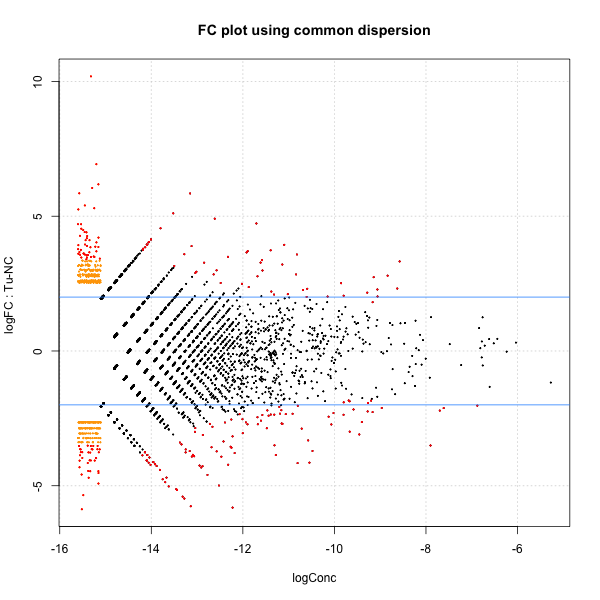
\includegraphics[height=0.45\textheight]{edgeR_case_study_Zhang-015.png}
\caption{Plot of the log-fold change against the log-concentration for
  each tag. The 243 most differentially expressed tags as identified
  by \edgeR~using the common dispersion are outlined in red.}
\label{fig:Zhang_FC1}
\end{center}
\end{figure}


\subsection{Analysing the data using moderated tagwise dispersions}
\subsubsection{Moderating the tagwise dispersion}
An extension to simply using the common dispersion for each tag is to
estimate the dispersion separately for each tag, while `squeezing'
these estimates towards the common dispersion estimate in order to
improve inference by sharing information between tags. This type of
analysis can also be carried out in few steps using the
\edgeR~package.

As noted earlier, the dispersion parameter is the overdispersion
relative to the Poisson, and represents the biological, or
sample-to-sample variability. The methods we developed moderate the
dispersion estimates towards a common dispersion, much like how the
\limma~package moderates the variances in the analysis of microarray
data.

The amount of moderation done is determined by the value of a weight
parameter \code{prior.n}. The value for \code{prior.n} corresponds to
the number of individual tags equivalent to the weight given to the
common likelihood. Thus, the higher \code{prior.n}, the more strongly
the individual dispersion estimates are moderated, or `squeezed',
towards the common value. To run the moderated analysis, we need to
determine how much moderation is necessary. How best to do this is
still an open research question, but we currently recommend selecting
a value for the weight parameter \code{prior.n} \emph{a priori} and
have found that very good results can be obtained this way.

In an experiment such as that we consider here, in which we have just
four samples, two in each group, and thus two degrees of freedom for
estimating the dispersion parameter. Standard tagwise dispersion
estimates are likely to be unreliable, so we want to give a reasonable
weight to the common likelihood. We need to choose a value for
\code{prior.n} such that individual tagwise dispersion estimates are
`squeezed' quite strongly towards the common dispersion. Here, we
choose a moderate amount of smoothing---we let \code{prior.n} be
$10$. This means that the common likelihood receives the weight of
$10$ individual tags, so there will be a reasonable degree of
`squeezing', but there is still ample scope to estimate an individual
dispersion for each gene.

The function \code{estimateTagwiseDisp} produces a DGEList object that
contains all of the elements present in the object produced by
\code{estimateCommonDisp}, as well as the value for \code{prior.n}
used (\code{d\$prior.n}) and the tagwise dispersion estimates
(\code{d\$tagwise.dispersion}), as we see below.

\begin{Schunk}
\begin{Sinput}
> d <- estimateTagwiseDisp(d, prior.n = 10)
\end{Sinput}
\begin{Soutput}
Using grid search to estimate tagwise dispersion. 
\end{Soutput}
\begin{Sinput}
> names(d)
\end{Sinput}
\begin{Soutput}
 [1] "samples"            "common.dispersion"  "prior.n"           
 [4] "tagwise.dispersion" "counts"             "pseudo.alt"        
 [7] "genes"              "all.zeros"          "conc"              
[10] "common.lib.size"   
\end{Soutput}
\begin{Sinput}
> head(d$tagwise.dispersion)
\end{Sinput}
\begin{Soutput}
[1] 1.0945 0.1317 0.0944 0.2144 0.1381 0.1580
\end{Soutput}
\end{Schunk}

It is interesting to consider the distribution of the tagwise
dispersion estimates. As we can see from the output below, the tagwise
dispersion estimates range from a minimum of $0.09$ to a maximum of
$1.09$. The range of dispersions is therefore large, but the tags in
the middle two quartiles of the tagwise dispersion estimates have
dispersion estimates close to the common dispersion estimate.

\begin{Schunk}
\begin{Sinput}
> summary(d$tagwise.dispersion)
\end{Sinput}
\begin{Soutput}
   Min. 1st Qu.  Median    Mean 3rd Qu.    Max. 
 0.0944  0.1720  0.1850  0.1990  0.2070  1.0900 
\end{Soutput}
\begin{Sinput}
> d$common.dispersion
\end{Sinput}
\begin{Soutput}
[1] 0.1969
\end{Soutput}
\end{Schunk}


\subsubsection{Testing}
The testing procedures when using tagwise dispersion estimates are
carried out exactly as for the common dispersion, as described above,
but we add the argument \code{common.disp=FALSE} to the call to
\code{exactTest}. Here we carry out the testing using the tagwise
dispersion estimates calculated using a \code{prior.n} value of ten.

\begin{Schunk}
\begin{Sinput}
> de.tgw <- exactTest(d, common.disp = FALSE)
\end{Sinput}
\begin{Soutput}
Comparison of groups:  Tu - NC 
\end{Soutput}
\end{Schunk}

The output below shows that when using tagwise dispersions, the
\edgeR~package still identifies a lot of differential expression
between the normal colon cell group and the primary CR cancer cell
group---indeed the $p$-values of the top tags are even smaller than
the top tags based on the common dispersion. This arises because the
moderated tagwise dispersions can be much smaller than the common
dispersion, and tags with smaller dispersions will have smaller
p-values than the same tags with $p$-values computed using a common
dispersion. As with the analysis using the common dispersion, all of
the top tags have a large fold change, indicating that these changes
in expression are likely to be biologically meaningful. We note that
the ranking is different, however, and not all of the top ten tags
according to using the common dispersion are found to be among the top
ten tags using tagwise dispersions.

\begin{Schunk}
\begin{Sinput}
> topTags(de.tgw)
\end{Sinput}
\begin{Soutput}
Comparison of groups: Tu-NC 
           logConc   logFC    PValue       FDR
AGCTGTTCCC  -27.95  44.129 1.571e-10 7.872e-07
TCACCGGTCA  -10.54  -4.144 2.009e-08 5.033e-05
GTCATCACCA  -30.15 -39.732 1.439e-07 1.950e-04
CTTGGGTTTT  -29.59  40.860 1.557e-07 1.950e-04
TAAATTGCAA  -10.81  -4.171 2.311e-07 2.317e-04
TAATTTTTGC  -13.15   5.840 5.265e-07 4.398e-04
GTGCGCTGAG  -30.36  39.306 7.671e-07 5.036e-04
ATTTCAAGAT  -13.16  -5.812 8.209e-07 5.036e-04
CTTGACATAC  -30.42 -39.197 9.042e-07 5.036e-04
TACAAAATCG  -29.96  40.103 1.484e-06 7.440e-04
\end{Soutput}
\end{Schunk}

The table below shows the raw counts for the tags that \edgeR~has
identified as the most differentially expressed using tagwise
dispersions. For these genes there seems to be very large differences
between the groups, suggesting that the DE genes identified are truly
differentially expressed, and not false positives.

We note that in general, when using tagwise dispersions, the counts
are more consistent within groups, as using tagwise dispersions
instead of the common dispersion penalises tags which are highly
variable within groups. The smaller the value selected for
\code{prior.n}, the more highly variable tags will be penalised, as
there is less `squeezing' of the tagwise dispersions towards the
common value. This effect is seen clearly in the table below (compare
this with the corresponding table for the analysis using the common dispersion).

\begin{Schunk}
\begin{Sinput}
> detags.tgw <- rownames(topTags(de.tgw)$table)
> d$counts[detags.tgw, ]
\end{Sinput}
\begin{Soutput}
             1  2   3    4
AGCTGTTCCC   0  0 119 1011
TCACCGGTCA 118 75   6    5
GTCATCACCA  35 20   0    0
CTTGGGTTTT   0  0  21   97
TAAATTGCAA 103 59   3    6
TAATTTTTGC   0  1  37   21
GTGCGCTGAG   0  0  18   23
ATTTCAAGAT  35 21   0    1
CTTGACATAC  18 20   0    0
TACAAAATCG   0  0  14   56
\end{Soutput}
\end{Schunk}

Of course, we can sort the top table differently, as we did earlier.

We see in the output below that $225$ genes are significantly
differentially expressed according to \edgeR~when using the tagwise
dispersion estimates (ten fewer than when using the common
dispersion). Of those tags, $84$ are up-regulated in the cancer cells
compared with the normal cells and $141$ are down-regulated in the
cancer cells compared with normal cells. These proportions of up- and
down-regulated tags are similar to those found using the common
dispersion, but there is a slightly higher proportion of
down-regulated tags in those identified as DE using tagwise
dispersions.

\begin{Schunk}
\begin{Sinput}
> sum(de.tgw$table$p.value < 0.01)
\end{Sinput}
\begin{Soutput}
[1] 225
\end{Soutput}
\begin{Sinput}
> toptgw <- topTags(de.tgw, n = sum(de.tgw$table$p.value < 0.01))
> sum(toptgw$table$logFC > 0)
\end{Sinput}
\begin{Soutput}
[1] 84
\end{Soutput}
\begin{Sinput}
> sum(toptgw$table$logFC < 0)
\end{Sinput}
\begin{Soutput}
[1] 141
\end{Soutput}
\end{Schunk}

Furthermore, we see below that $76$ tags ($1.5$\% of the total
number) have a $p$-value of less than $0.05$ after adjusting for
multiple testing using the~\citet{Benjamini95} method for controlling
the FDR, which is strong evidence for differential expression.

\begin{Schunk}
\begin{Sinput}
> summary(decideTestsDGE(de.tgw, p.value = 0.05))
\end{Sinput}
\begin{Soutput}
   [,1]
-1   47
0  4936
1    29
\end{Soutput}
\end{Schunk}


\subsubsection{Visualising DGE results}
Shown below is the code for producing the default fold-change plot
using \code{plotSmear} with the DE tags as determined using tagwise
dispersions highlighted, and the result of this code is shown in
Figure~\ref{fig:Zhang_FC2}.

\begin{Schunk}
\begin{Sinput}
> detags.tgw <- rownames(topTags(de.tgw, n = sum(de.tgw$table$p.value < 
+     0.01))$table)
> png(file = "edgeR_case_study_Zhang-028.png", height = 600, width = 600)
> plotSmear(d, de.tags = detags.tgw, main = "FC plot using tagwise dispersions")
> abline(h = c(-2, 2), col = "dodgerblue")
> dev.off()
\end{Sinput}
\begin{Soutput}
null device 
          1 
\end{Soutput}
\end{Schunk}

In Figure~\ref{fig:Zhang_FC2}, the $225$ tags identified as
differentially expressed (i.e.~those identified as significant
($p$-value less than $0.01$) by \edgeR~using the tagwise dispersions)
are highlighted in red. We see that the pattern of differential
expression using tagwise dispersions that we see in
Figure~\ref{fig:Zhang_FC2} is very similar to that obtained using the
common dispersion that we saw in Figure~\ref{fig:Zhang_FC1}.

\begin{figure}[ht]
\begin{center}
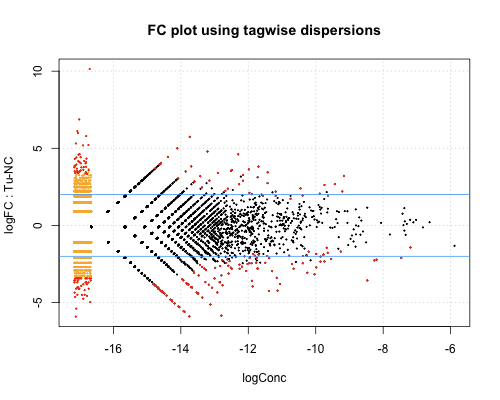
\includegraphics[height=0.45\textheight]{edgeR_case_study_Zhang-028.png}
\caption{Plot of the log-fold change against the log-concentration for
  each tag. The 225 most differentially expressed tags as identified
  by \edgeR~are outlined in red.}
\label{fig:Zhang_FC2}
\end{center}
\end{figure}

\subsection{Setup}
This analysis of \citet{Zhang:1997p13}'s SAGE data was conducted on:
\begin{Schunk}
\begin{Sinput}
> sessionInfo()
\end{Sinput}
\begin{Soutput}
R version 2.13.0 beta (2011-03-30 r55205)
Platform: i386-apple-darwin9.8.0/i386 (32-bit)

locale:
[1] C/UTF-8/C/C/C/C

attached base packages:
[1] stats     graphics  grDevices utils     datasets  methods   base     

other attached packages:
[1] edgeR_2.1.16

loaded via a namespace (and not attached):
[1] limma_3.7.26
\end{Soutput}
\end{Schunk}
and took 2--3 minutes to carry out on an Apple MacBook with a 2.8
Ghz Intel Core 2 Duo processor and 8 Gb of 1067 MHz DDR3 memory.


